\section{Operating Modes}

The UART module is designed for full–duplex asynchronous serial communication. It implements independent transmitter (TX) and receiver (RX) paths that operate concurrently. Both paths include configurable settings for baud rate, data length, and parity. In addition, each side incorporates an internal dynamic FIFO buffer to decouple external data handling from the serial transmission or reception. This section describes the operating modes of the UART module in detail.

\begin{figure}[H]
    \centering
    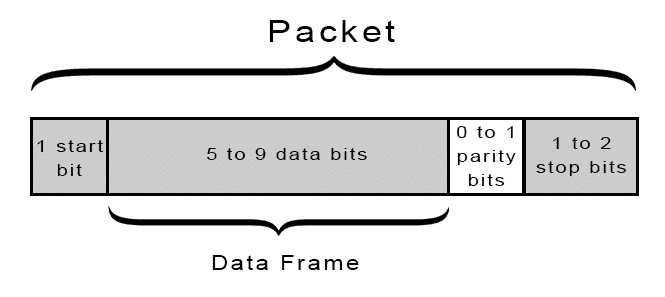
\includegraphics[width=0.85\textwidth]{images/frame_format.png}
    \caption{Frame Formats}
    \label{fig:frame_formats}
  \end{figure}
  
\subsection{Transmitter Mode}

When operating in transmitter mode, the UART transmitter performs the following functions:

\begin{itemize}
    \item \textbf{Data Buffering:} 
    \begin{itemize}
        \item Software writes data into the \texttt{TX\_DATA\_IN} register.
        \item A write trigger (e.g., pulsing \texttt{TX\_LOAD} or \texttt{txDataRegWrite}) pushes the word into an internal dynamic FIFO. The FIFO depth is parameterized by \texttt{bufferSize}.
        \item The transmitter state machine automatically pops data from the FIFO when a transmission is ready.
    \end{itemize}
    
    \item \textbf{Baud Rate Updating:}
    \begin{itemize}
        \item The TX path includes a dedicated \texttt{UartBaudRateGenerator} module.
        \item Software sets the desired baud rate and clock frequency via registers (\texttt{TX\_BAUD\_RATE} and \texttt{TX\_CLOCK\_FREQ}) and then pulses the update control (e.g., \texttt{TX\_UPDATE\_BAUD}).
        \item The transmitter enters a \texttt{BaudUpdating} state. The baud generator computes the effective \texttt{clocksPerBit} (i.e. the number of system clocks per transmitted bit) and asserts a \texttt{baudValid} signal when complete.
        \item Once valid, the computed divisor is stored in \texttt{clocksPerBitReg} and the state machine transitions back to \texttt{Idle}.
    \end{itemize}
    
    \item \textbf{Data Transmission:}
    \begin{itemize}
        \item Upon detecting that data is available in the FIFO and the transmitter is idle, the state machine initiates a new transmission by loading the next word from the FIFO.
        \item Before transmission begins, the TX data word is “reversed” (using an internal \texttt{reverse()} function) so that the least-significant bit (LSB) is transmitted first.
        \item The transmission sequence then follows standard UART timing:
            \begin{enumerate}[noitemsep]
                \item \textbf{Start Bit:} A start bit (\texttt{0}) is driven.
                \item \textbf{Data Bits:} The state machine shifts out the configured number (\texttt{TX\_NUM\_OUTPUT\_BITS\_DB}) of data bits in the \texttt{Data} state.
                \item \textbf{Parity Bit (Optional):} If parity is enabled (\texttt{TX\_USE\_PARITY\_DB}=1), a parity bit is computed from the full (unshifted) data word and transmitted in the \texttt{Parity} state. The selection of odd or even parity is controlled by \texttt{TX\_PARITY\_ODD\_DB}.
                \item \textbf{Stop Bit:} Finally, one or more stop bits (\texttt{1}) are transmitted in the \texttt{Stop} state.
            \end{enumerate}
        \item During transmission, the TX output (\texttt{tx}) is driven accordingly. When idle, \texttt{tx} remains high.
    \end{itemize}
    
    \item \textbf{State Machine Overview:}
    \begin{itemize}
        \item The TX state machine transitions through the following key states:
            \begin{itemize}
                \item \texttt{Idle}: Waiting for new data and/or baud update.
                \item \texttt{BaudUpdating}: Waiting for the baud rate generator to compute \texttt{clocksPerBit}.
                \item \texttt{Start}: Driving the start bit.
                \item \texttt{Data}: Shifting out the data bits.
                \item \texttt{Parity}: (Optional) Transmitting the parity bit.
                \item \texttt{Stop}: Driving the stop bit(s) before returning to \texttt{Idle}.
            \end{itemize}
        \item The signal \texttt{startTransaction} is generated when a new word is ready (from FIFO) and the transmitter is idle.
        \item The computed \texttt{clocksPerBit} governs the timing of data sampling and shifting.
    \end{itemize}
\end{itemize}

\subsection{Receiver Mode}

In receiver mode, the UART receiver continuously monitors the \texttt{rx} input and performs the following functions:

\begin{itemize}
    \item \textbf{Signal Synchronization:}
    \begin{itemize}
        \item The asynchronous \texttt{rx} input is first passed through a chain of flip–flops (of depth defined by \texttt{syncDepth}) to mitigate metastability.
        \item The synchronized signal (\texttt{rxSync}) is used for all subsequent sampling.
    \end{itemize}
    
    \item \textbf{Baud Rate Updating:}
    \begin{itemize}
        \item Similar to the transmitter, the RX path uses a \texttt{UartBaudRateGenerator}.
        \item Software sets the RX baud rate and clock frequency using registers (e.g., \texttt{RX\_BAUD\_RATE} and \texttt{RX\_CLOCK\_FREQ}) and then pulses \texttt{RX\_UPDATE\_BAUD}.
        \item The RX state machine enters a \texttt{BaudUpdating} state, during which the effective \texttt{clocksPerBit} is calculated and stored in \texttt{clocksPerBitReg}.
        \item Once the baud generator asserts \texttt{baudValid}, the FSM transitions back to \texttt{Idle} and resumes monitoring.
    \end{itemize}
    
    \item \textbf{Data Reception:}
    \begin{itemize}
        \item The receiver continuously samples the \texttt{rxSync} signal.
        \item A falling edge (transition from high to low) indicates a start bit, and the receiver then enters the \texttt{Start} state.
        \item After a fixed delay (approximately half the duration of a bit period), the receiver begins to sample the incoming data bits in the \texttt{Data} state.
        \item If parity is enabled (\texttt{RX\_USE\_PARITY\_DB}=1), the FSM transitions to the \texttt{Parity} state and compares the received parity bit against the expected value. The expected parity is computed from the shifted–in data and the setting of \texttt{RX\_PARITY\_ODD\_DB}.
        \item Finally, the receiver checks the stop bit in the \texttt{Stop} state. If the stop bit is not detected (i.e., if the line is not high at the end of the bit period), a framing error is flagged.
    \end{itemize}
    
    \item \textbf{Data Buffering:}
    \begin{itemize}
        \item Once a complete frame is successfully received (with no errors), the RX data is latched and then pushed into an internal dynamic FIFO.
        \item This FIFO, whose depth is set by the \texttt{bufferSize} parameter, allows the receiver to decouple the hardware reception rate from the software read rate.
        \item Software can later pop data from the RX FIFO by asserting the read control signal (e.g., \texttt{rxDataRegRead}).
    \end{itemize}
    
    \item \textbf{State Machine Overview:}
    \begin{itemize}
        \item The RX state machine progresses through the following states:
            \begin{itemize}
                \item \texttt{Idle}: Waiting for a start bit.
                \item \texttt{BaudUpdating}: If new baud settings are provided.
                \item \texttt{Start}: Confirming the start bit.
                \item \texttt{Data}: Shifting in the data bits.
                \item \texttt{Parity}: (Optional) Sampling and checking the parity bit.
                \item \texttt{Stop}: Verifying the stop bit.
            \end{itemize}
        \item Upon successful reception, the received word is transferred to the FIFO. If errors occur (e.g., parity, stop bit, or overrun errors), error flags in \texttt{UartRxError} are updated.
    \end{itemize}
\end{itemize}

\subsection{Simultaneous Operation}

Both transmitter and receiver operate in parallel under full–duplex conditions. They use independent state machines and FIFOs, allowing transmission and reception to occur simultaneously without interference. The APB interface provides separate control and status registers for TX and RX, so software can configure and monitor each path independently.

\subsection{Error Handling}

The UART module includes robust error detection mechanisms:
\begin{itemize}
    \item \textbf{Parity Error:} If parity checking is enabled and the received parity bit does not match the computed value, the RX FSM flags a parity error.
    \item \textbf{Framing (Stop Bit) Error:} If the expected stop bit is not detected (i.e., the line is not high during the stop bit period), a framing error is flagged.
    \item \textbf{Overrun Error:} If a new frame is received before the previous data is read from the RX FIFO, an overrun error may be reported.
    \item \textbf{Baud Rate Update Errors:} If the new baud configuration results in an invalid \texttt{clocksPerBit} calculation (or if parameters are out of range), a top–level error flag (e.g., \texttt{TOP\_ERROR}) can be asserted.
\end{itemize}
Error flags are accessible via dedicated status registers and are cleared by writing to specific error–clear registers.

\subsection{Summary}

In summary, the UART module’s operating modes include:
\begin{itemize}
    \item \textbf{Transmitter Mode:} 
    \begin{itemize}
        \item Uses a dynamic FIFO for buffering outgoing data.
        \item Employs a state machine that transitions through Idle, BaudUpdating, Start, Data, (optional) Parity, and Stop states.
        \item Features an internal data reversal function to ensure LSB-first transmission.
    \end{itemize}
    \item \textbf{Receiver Mode:} 
    \begin{itemize}
        \item Samples an asynchronously synchronized RX line.
        \item Uses a similar state machine (Idle, BaudUpdating, Start, Data, (optional) Parity, Stop) to capture incoming data.
        \item Pushes successfully received data into an internal dynamic FIFO for later software access.
    \end{itemize}
    \item \textbf{Full-Duplex Operation:} TX and RX operate independently yet concurrently, allowing simultaneous transmission and reception.
    \item \textbf{Error Handling:} Parity, framing, and overrun errors are detected and flagged for software intervention.
\end{itemize}
